% Template for NIME 2013
%
% Modified by Kyogu Lee on 7 October 2012
%
% Modified by Georg Essl on 7 November 2011
%
% Based on "sig-alternate.tex" V1.9 April 2009
% This file should be compiled with "nime2011.cls"
%

\documentclass{nime-alternate}

\begin{document}
%
% --- Author Metadata here ---
\conferenceinfo{NIME'13,}{May 27 -- 30, 2013, KAIST, Daejeon, Korea.}

\title{KIB: Simplifying Gestural Instrument Creation using Widgets}

%
% You need the command \numberofauthors to handle the 'placement
% and alignment' of the authors beneath the title.
%
% For aesthetic reasons, we recommend 'three authors at a time'
% i.e. three 'name/affiliation blocks' be placed beneath the title.
%
% NOTE: You are NOT restricted in how many 'rows' of
% "name/affiliations" may appear. We just ask that you restrict
% the number of 'columns' to three.
%
% Because of the available 'opening page real-estate'
% we ask you to refrain from putting more than six authors
% (two rows with three columns) beneath the article title.
% More than six makes the first-page appear very cluttered indeed.
%
% Use the \alignauthor commands to handle the names
% and affiliations for an 'aesthetic maximum' of six authors.
% Add names, affiliations, addresses for
% the seventh etc. author(s) as the argument for the
% \additionalauthors command.
% These 'additional authors' will be output/set for you
% without further effort on your part as the last section in
% the body of your article BEFORE References or any Appendices.

\numberofauthors{1} %  in this sample file, there are a *total*
% of EIGHT authors. SIX appear on the 'first-page' (for formatting
% reasons) and the remaining two appear in the \additionalauthors section.
%
\author{
% You can go ahead and credit any number of authors here,
% e.g. one 'row of three' or two rows (consisting of one row of three
% and a second row of one, two or three).
%
% The command \alignauthor (no curly braces needed) should
% precede each author name, affiliation/snail-mail address and
% e-mail address. Additionally, tag each line of
% affiliation/address with \affaddr, and tag the
% e-mail address with \email.
%
% 1st. author
\alignauthor Edward Zhang\\
       \affaddr{Princeton University}\\
       \affaddr{Princeton, NJ}\\
       \email{edwardz@princeton.edu}
}
\maketitle
\begin{abstract}
The Microsoft Kinect is a popular and versatile input device for musical interfaces.
However, using the Kinect for such interfaces requires not only significant programming
experience, but also the use of complex geometry or machine learning techniques to translate joint
positions into higher level gestures. We created the Kinect Instrument Builder (KIB) to
address these difficulties by structuring gestural interfaces as combinations of gestural
widgets. KIB allows the user to design an instrument by configuring gestural primitives,
each with a set of simple but exciting visual feedback elements. After designing an instrument
on KIB's web interface, users can play the instrument on KIB's performance interface, 
which displays visualizations and transmits OSC messages to other applications for sound synthesis
or further remapping.
\end{abstract}

\keywords{Kinect, gesture, widgets, OSC, mapping}

\section{Introduction}
New technology has enabled the development of many types of novel interfaces for digital
musical instruments (DMIs). One of the most versatile is the gestural interface. In comparison
with traditional interfaces, gestural systems allow for increased complexity with more degrees
of freedom. The Microsoft Kinect is an inexpensive, commercially available sensor that has been
extremely popular for gestural interfaces because of its depth camera and joint tracking
capabilities. A search for ``instrument'' or ``music'' at KinectHacks
\footnote{http://www.kinecthacks.net} provides
several pages worth of musical interfaces designed by the programming community; even in the
academic world, four papers presented at NIME 2012 used the Kinect sensor \cite{nimekinect1, nimekinect2, nimekinect3, digito}. The Kinect has been used in compelling performances
such as in the Vmotion system\footnote{http://www.custom-logic.com/blog/v-motion-project-the-instrument/} that showcase the potential of gestural instruments.

However, designing gestural interfaces that use the Kinect presents several challenges. 
Firstly, creating such interfaces requires a good deal of programming knowledge to create
applications that can communicate with the Kinect and access its depth and skeletal tracking streams. 
Fortunately, several existing systems, such as \cite{yoo2011creating} and osceleton\footnote{https://github.com/Sensebloom/OSCeleton}, take the output from
the Kinect and broadcast MIDI or OSC messages containing the skeletal coordinate data. However,
the more difficult problem of translating raw joint positions into meaningful gestures remains.
Developers often have to use complicated machine learning, computer vision, or geometrical
techniques to turn skeletal data into a form suitable for use in musical interfaces. 

In order to simplify this process, we designed the Kinect Instrument Builder (KIB) around the
concept of gestural widgets. Widget-based interfaces have been fairly successful for multitouch
surfaces, especially in commercial systems such as in touchOSC\footnote{http://hexler.net/software/touchosc}. In these interfaces, intuitive visual elements provide feedback for interactions
with knobs, sliders, buttons, and more abstract widgets; each widget sends its own OSC messages
which can be used in sound synthesis software, such as ChucK, PureData, or Max/MSP. By applying
the same principles to gestural interfaces that use the Microsoft Kinect, we hope to make gestural
instrument design simpler and more accessible. 

\section{Background}
\subsection{Widget-based Interface Design}
The physical controls used in sound editing systems form the inspiration for multitouch
widget-based interfaces such as Argos \cite{diakopoulos2010argos}, TouchOSC, 
Lemur\footnote{http://www.jazzmutant.com/lemur\_overview.php}, and Konkreet Performer\footnote{http://konkreetlabs.com/}. These systems are purely
input interfaces and do not on their own perform any sound synthesis; they communicate user input event information through
protocols such as MIDI and OSC\cite{osc}.

The JazzMutant Lemur, released in 2005, was the
first successful commercial multitouch widget-based system. Lemur was based around a custom-built multitouch device. Users would design their own interfaces
on the desktop and then interact with these interfaces on the touchscreen. In
addition to physically inspired widgets such as buttons and sliders, Lemur also provided
several nontraditional widgets with their own unique behavior and visual elements. 

TouchOSC is a similar system to Lemur, but does not require the use of specialized hardware.
TouchOSC provides a desktop
application that allows users to design interfaces out of combinations of widgets for use on
multitouch mobile devices. Its low cost and availability for consumer devices running iOS and Android have
made the specialized capabilities of the JazzMutant Lemur accessible to everyone.

Konkreet Performer moves away from the physically based sliders and knobs of TouchOSC and the
Lemur, instead focusing their interface on a new type of widget. A single input element consists of several
individual nodes; these nodes can be rotated, moved, or zoomed. Each property of each node is an independent variable sent over OSC or MIDI. Konkreet Performer places a high importance on visual feedback, both
as a performer tool and as an audience engagement mechanism. It allows users to 
customize the appearance of the nodes and elements onscreen. Konkreet also is developing a 
separate application, Konkreet Visualizer, to augment visual elements of a musician's interaction with Konkreet Performer for an audience. Visual feedback is
vital for natural user interfaces \cite{bravenuiworld}, and is especially important for engaging audiences when performers are using unfamiliar interfaces. KIB shares this prioritization of visual feedback, both for the performer and the audience. 

Several academic systems have also been developed to explore the capabilities of multitouch
widget-based systems. In contrast to existing commercial systems, Control was designed for maximum scriptability, with interfaces and logic written using web technologies such as HTML, CSS, and Javascript. Control also takes advantage of the many sensors on mobile devices such
as the microphone and accelerometer, in addition to the multitouch screen \cite{roberts2011control}. In a later work, Control is 
extended to automate the connection between an instance of Control and a synthesis engine in Max, LuaAV\cite{wakefield2010luaav}, or SuperCollider\footnote{http://supercollider.sourceforge.net/} \cite{roberts2012mobile}.

\subsection{Gestural Widgets}
Gestural control systems are fairly new and few works conceptualize gestural interactions in terms of widgets. Berthaut et al investigate 3D widgets in virtual environments for musical
interfaces, but are focused on interaction within immersive virtual environments \cite{berthaut2011interacting}. This system uses a Wii remote to provide tactile feedback through vibration,
audio feedback through a small speaker, and input through buttons, orientation, and position. The combination of immersive visual feedback and tactile feedback made the abstraction
of interacting with geometric widgets much more intuitive.

Microsoft's Kinect for Windows SDK\footnote{http://www.microsoft.com/en-us/kinectforwindows/develop/learn.aspx} provides several simple gesture detectors such as swipe left and
swipe right, but the selection is very limited. Several libraries have provided generic gesture recognition toolkits such as the Kinect Toolbox\footnote{http://kinecttoolbox.codeplex.com/}, but these have been focused on gesture training and recognition, rather
than determining a fundamental set of gestures for interaction. We hope that, in our
experiments with KIB, we will gain a better understanding of what movement types form good gestural primitives.
\section{Implementation}
%FIXME: Implementation
KIB consists of two distinct components. The instrument design interface is a web
application that allows the user to rapidly construct a widget-based instrument. The user
can save the resulting instrument and play it using the performance interface. The source code
for both components is available on GitHub\footnote{https://github.com/kyzyx/KIB}.
\subsection{Gestural Widgets}
Since the central concept of KIB is the gestural widget, the set of widgets must be chosen
carefully. We provided seven simple widget types; these types can be divided into streaming
widgets, which provide data updates at every frame of Kinect data, and instantaneous widgets,
which trigger once a certain event happens.
\begin{figure}
	\centering
		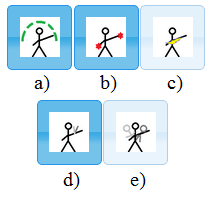
\includegraphics[width=0.6\columnwidth]{figures/icons.png}
	\caption{Icons for streaming widgets. a) Arc widget, b) Hands widget, c) Ball widget
    d) Wave widget e) Body widget}
	\label{fig:widgeticons}
\end{figure}

\begin{itemize}
\item The \textbf{Arc} widget can be used as a combination of a streaming and instantaneous widget.
Inspired by elements in the Vmotion system, this widget places an arch around the user that is 
activated when their arms are at full extension. Although tiring, this makes it easier for the 
user to feel when the widget is activated. The arch can be divided into several sections (as in
Figure~\ref{fig:widgeticons}a); if the arm activates the arc inside one of these sections, an
appropriate instantaneous event is generated. If the arc is not divided, then the widget will
stream the angle at which each arm intersects the arc.
\item The \textbf{Hands} widget simply streams the raw coordinates from the Kinect skeletal 
data to the synthesis engine. We chose to use this raw data because the hands are the
most important body part for performing gestures, and raw coordinates are a versatile way to
create simple continuous mappings.
\item The \textbf{Wave} widget streams the angle between the forearm and the upper arm. One
way to conceive of this widget is a giant knob centered on the elbow. One or both arms can
be tracked by this widget.
\item When using the \textbf{Ball} widget, we imagine the user to be holding a ball. The widget streams
the size of the ball (the distance between the hands) as well as the orientation of the ball
(the angle that the line between the hands forms with the ground). A similar widget appears
in the Vmotion system.
\item The \textbf{Body} widget is unique in that it does not involve the arms. Instead, this
widget looks at the angle the torso forms with the ground. More specifically, it takes the
vector from the center of the hips to the head and determines the angle this vector forms
with the horizontal. Since the other widgets all involve the hands and arms, they often
are difficult to control independently; this widget gives the user an alternate body part for interaction.
\item The \textbf{Punch} is an instantaneous widget. It is activated when the user's arm is
fully extended in the forward direction ($-z$ direction in Kinect coordinates). We use hysteresis to control the triggering state; this means that the $z$-distance
between the extended arm and the body must cross above threshold
distance to activate the widget, and then must pass below a lower threshold to reenable
activation. Note that no arm speed constraint is added, so in theory one could punch
very slowly and still activate the widget; the hysteresis is included to prevent a slow or 
static arm extension from continuously triggering the widget.
\item The \textbf{Clap} is an instantaneous widget. It is activated when the distance
between the user's hands crosses below some threshold. Similar to the \textbf{Punch} widget,
it uses hysteresis to control the activation of the widget.
\end{itemize}

These gestures are based on simple geometry and thresholding; we anticipate that more complex
gestural primitives might require the use of machine learning techniques for recognition. Most
of these widgets assume the user stays standing in approximately the same
location. This assumption rests on the limitations of the Kinect's skeletal tracking system,
as well as the limited field of view of the static Kinect sensor.
\subsection{Kinect Instrument Structure}
We refer to a combination of active widgets and the associated visualizations as a 
\textit{kiblet}. A complete performance with a Kinect instrument might involve a series 
of kiblets, each active at different times. The performer switches between kiblets via a
configurable trigger system. Kiblets can be triggered to activate at a certain time during the
performance, upon a certain widget event such as a Punch, or when the performance interface
receives a custom OSC control message. 

This hierarchical structure involving widgets and kiblets was inspired by TouchOSC and the Vmotion 
performance. Vmotion is one of the few professionally designed performance interfaces that use the Kinect,
so many of our design decisions borrowed from its structure. In particular, we note that having many
widgets active at once greatly increases complexity and often overloads both the performer and
the audience; however having too few widgets limits the range of possibilities for a long
performance. Being able to switch between interfaces is a way to combine the simplicity of
fewer widgets while keeping the flexibility of KIB's widgets available during a performance. 
TouchOSC provides several interfaces that the user can easily switch between during performance
as well.

\subsection{Instrument Design Interface}
\begin{figure}
	\centering
		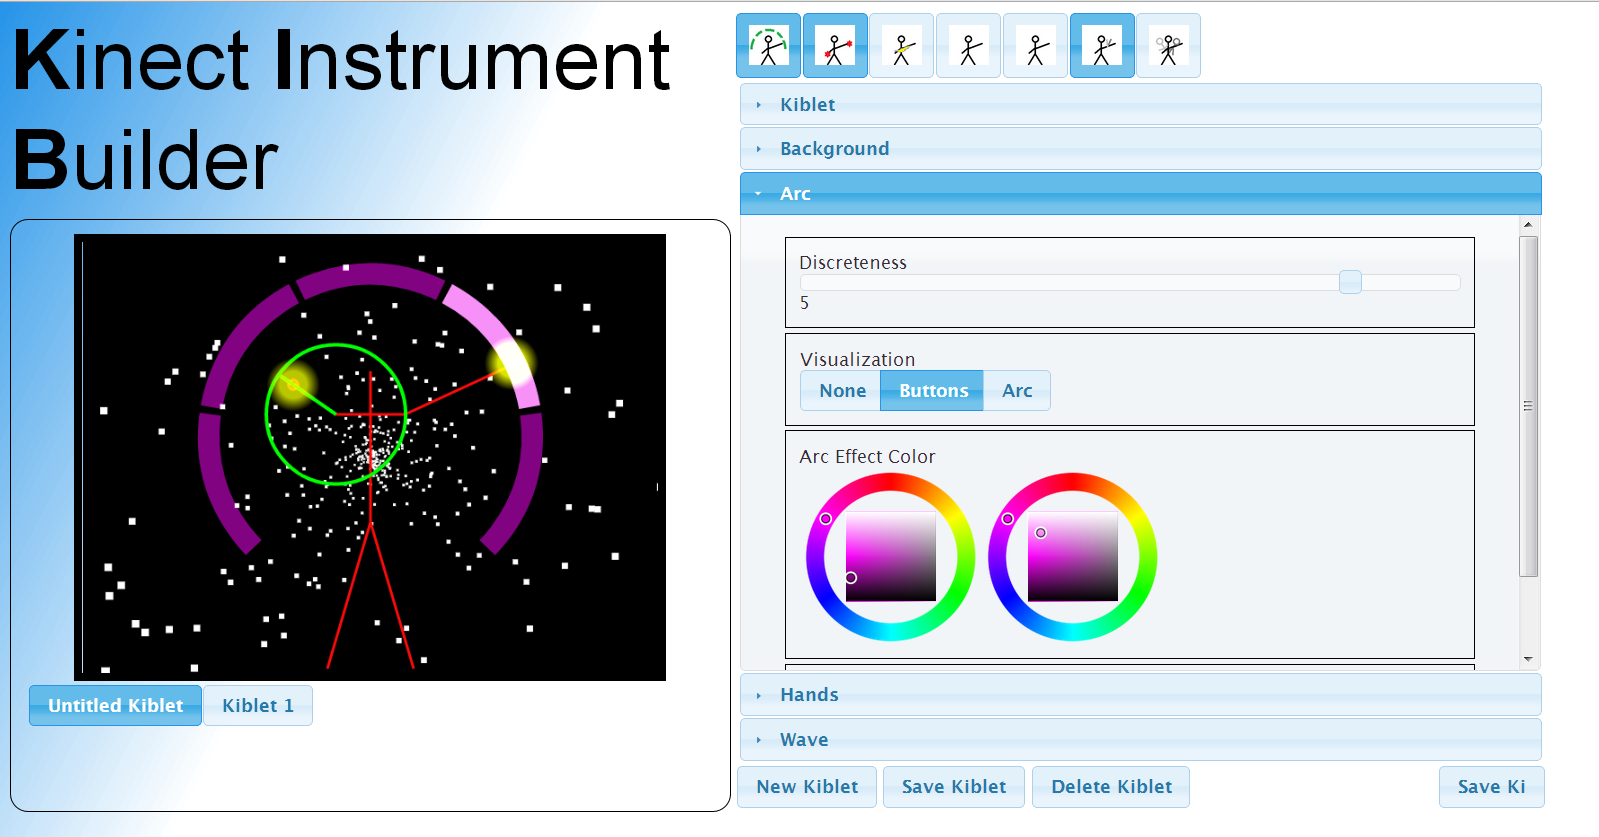
\includegraphics[width=1\columnwidth]{figures/kib.png}
	\caption{Instrument design interface}
	\label{fig:interface}
\end{figure}

The instrument design interface is a web interface. It is written in Javascript,
HTML, and CSS. This ensures a lightweight, platform-independent graphical user interface
with rich interactive elements.

One side of the interface provides an approximate visualization of the current kiblet. It shows the visual
elements for the background and user avatar, as well as any visualizations for the widgets
in the current kiblet. This interface is also interactive - the user can drag the avatar's head or hands
into different positions to see how the visualization changes with user movement in performance. A list of the kiblets in the current instrument is displayed under the visualization, so
that the user can switch between kiblets.

The other side of the interface allows the user to configure the kiblet, widgets, and visualization.
Buttons depicting the available widgets are displayed at the top of the window; these buttons will be
slightly shaded if the widget is currently active in the kiblet. Beneath that, a panel provides a list of
settings the user can use to design the visualizations for the widget and kiblet, as well as customize logistical
parameters such as OSC message names, widget data resolution, and kiblet trigger conditions.

The user can save the resulting instrument by clicking the ``Save KI'' button, which will open
a new window containing the configuration file generated from the design. This configuration
file is encoded in JSON and is used as input to the performance interface.
\subsection{Performance Interface}
The performance interface is a Windows application written in C++. Unfortunately, the Kinect
for Windows SDK is not cross-platform, and other Kinect APIs such as freenect\footnote{http://openkinect.org/wiki/Main\_Page} and OpenNI\footnote{http://www.openni.org/} do not yet support
the Kinect for Windows sensor. Therefore the KIB performance interface is currently restricted
to running on Microsoft Windows. The performance application uses the SDL library\footnote{http://www.libsdl.org/} and OpenGL
for visualization, and the oscpack\footnote{http://code.google.com/p/oscpack/} library for
OSC networking. 

\begin{figure}
	\centering
		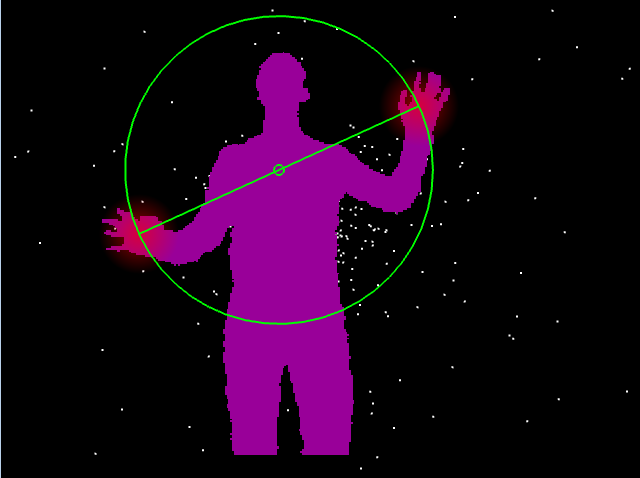
\includegraphics[width=1\columnwidth]{figures/player.png}
	\caption{Performance Interface Visualization. This shows the visualization for a kiblet
that has the Ball and Hands widgets activated. The background is a starfield and the avatar
representation is a silhouette of the performer.}
	\label{fig:player}
\end{figure}

At each frame of data from the Kinect, each widget in the active kiblet has the opportunity to process 
the Kinect data and use it to render a visualization and send an OSC message. These messages
have a standardized form outlined in Table~\ref{tab:osc}.
While the visualizations for widgets will generally use only the skeletal data given by the
Kinect SDK, the background and avatar visualizations can use the actual RGB or depth streams
that the Kinect provides; for example, in Figure~\ref{fig:player} the avatar presented uses the user's
silhouette as sensed by the Kinect. 

\begin{table*}
\centering
\caption{OSC Message Formats. i denotes integer value, f denotes floating-point value. All coordinates are in meters, while all angles are in radians.}
\begin{tabular}{|c|c|c|p{0.3\textwidth}|} \hline
\textbf{Widget Type} & \textbf{Continuous/Instantaneous} & \textbf{OSC Message Format} & \textbf{Contents}\\ \hline
Arc (Discrete) & Instantaneous & i & Section of arc activated\\ \hline
Arc (Continuous) & Continuous & f f& Angle of right arm and left arm intersection with arc; $-2\pi$ if arm not intersecting arc\\ \hline
Hands & Continous & f f f f f f & $x,y,z$ coordinates of right hand followed by $x,y,z$ coordinates of left hand, relative to Kinect \\ \hline
Wave & Continuous & f f & Angle between the horizontal and the right and left forearm; $-2\pi$ if arm not tracked\\ \hline
Ball & Continuous & f f & Distance between hands, and the angle between the hands
and the horizontal\\ \hline
Body & Continuous & f & Angle between the vertical and the line between the head and hips\\ \hline
Punch & Instantaneous & None & N/A \\ \hline
Clap & Instantaneous & None & N/A \\ \hline
\end{tabular}
\label{tab:osc}
\end{table*}

In the current implementation,
the thresholds for instantaneous events are tuned by hand to minimize latency; however in the
future it may be beneficial for these thresholds to be adjustable by the user. The Kinect provides
data at a peak rate of 30 frames per second.

\section{Evaluation}
Several potential users of our interface experimented with the prototype system. They were
given the opportunity to write their own sound synthesis scripts, or were provided a basic
set of synthesis scripts written in ChucK. We conducted informal interviews to assess the
usability of KIB and the satisfaction with the instruments that could be designed with KIB. We
especially were interested in their opinions on the selection of widgets and whether there
were any other gestural primitives they would like to use.
\section{Discussion}
The most important question KIB raises is whether decomposing gestural instruments into a
set of widgets is a useful abstraction. While more technical or creative performers may wish
to stretch the possibilities of a gestural instrument, we have seen from works such as Vmotion
that impressive results can be gained even from simple widgets. For the general user, 

Another common issue was the separation between widget output and appropriate parameters for
sound synthesis. Although KIB handles the mapping from raw joint data to gestural data, the
step of mapping from gestural data to sound synthesis parameters is still required. This means
that the composer or performer must be familiar with the specifics of the OSC messages passed
and the meaning of the data it provides, which is not ideal.
\section{Conclusion}
%FIXME: Conclusion

% The following two commands are all you need in the
% initial runs of your .tex file to
% produce the bibliography for the citations in your paper.
\bibliographystyle{abbrv}
\bibliography{kib-references}  % sigproc.bib is the name of the Bibliography in this case
% You must have a proper ".bib" file
%  and remember to run:
% latex bibtex latex latex
% to resolve all references
%
% ACM needs 'a single self-contained file'!
\end{document}
